\chapter{Снижение размерности динамической модели нефтегазового месторождения}\label{ch:ch2}

% \{TODO nomenclature}

\newcommand{\bvec}[1]{\mathbf{#1}}
\newcommand{\resid}{\bvec{r}}
\newcommand{\unk}{\bvec{u}}
\newcommand{\jac}{\mathrm{J}}
\newcommand{\dunk}{\Delta \unk}
\newcommand{\vunk}{\bvec{v}}
\newcommand{\matr}[1]{\mathrm{\uppercase{#1}}}
\newcommand{\norm}[2][~]{\left\| #2  \right\|_{#1}}
\newcommand{\transpose}[1]{\matr{#1}^\mathrm{T}}
\newcommand{\dvunk}{\Delta \vunk}
\newcommand{\deriv}[3][]{\frac{\partial^{#1} #2}{\partial #3^{#1}}}
\newcommand{\pc}[1][~]{\bvec{\varphi}_{#1}}
\newcommand{\param}{\bvec{\mu}}
\newcommand{\nlin}{\bvec{\eta}}

В данной главе описаны рассматриваемые в работе определяющие уравнения, представляющие интерес в сфере нефтегазового моделирования, базовые методы эмпирического низкоразмерного моделирования и соответствующие положения о подходе к построению таких моделей.

\section{Определяющие уравнения}

\subsection{Система уравнений чёрной нефти}

Широко используемой моделью течения многофазного флюида в пористой среде, на которую воздействует система скважин, является система уравнений чёрной нефти  с источниковыми членами по формуле Писмана.

\begin{multline}
    \label{eq:blackoil}
    \deriv{~}{t}\left(
        \varphi \matr{R}_{\alpha A} \frac{s_A}{b_A}
    \right) - \overrightarrow{\nabla} \left[
        \matr{R}_{\alpha A} \left(
            K\frac{\kappa_A}{\mu_A b_A}\nabla p
        \right)
    \right] \\
    = \matr{R}_{\alpha A}
    \frac{2\pi K \kappa_A}{\mu_A b_A \ln(r_c r_\text{well}^{-1})}
    \left(p - p_\text{well}\right)
\end{multline}

\begin{align}
    \label{eq:sats}
    \sum_A s_A = 1
\end{align}

Соотношение~\ref{eq:blackoil} представляет собой уравнение неразрывности потока многофазного многокомпонентного флюида с замыкающим соотношением нормировки насыщенностей фаз~\ref{eq:sats}.
В численных экспериментах в работе использовалась в том числе конечно-разностная дискретизация модели черной нефти в программной библиотеке MATLAB Reservoir Simulation Toolbox (MRST).

\subsection{Модельная задача}

В численных экспериментах так же используется модельная задача нелинейной диффузии в одномерном пространстве, замкнутая начальным условием и краевыми условиями Дирихле.

\begin{equation} \label{eq:diffusion}
   u(x,t): \deriv{u}{t} - \deriv{}{x} \left[\kappa(x, u) \deriv{u}{x} \right]= q \delta (x - x_q)
\end{equation}

Свойства этого модельного уравнения характеры так же и для поля давлений в уравнении~\ref{eq:blackoil}: это нестационарный диффузионный процесс в однородной среде с точечным источником. Более того, система уравнений чёрной нефти принимает аналогичный вид в приближении однофазного течения в одномерной среде.

В численных экспериментах задача решалась численно полностью неявной схемой с конечно-разностной пространственной дискретизацией.

\begin{figure}[ht]
    \centerfloat{
        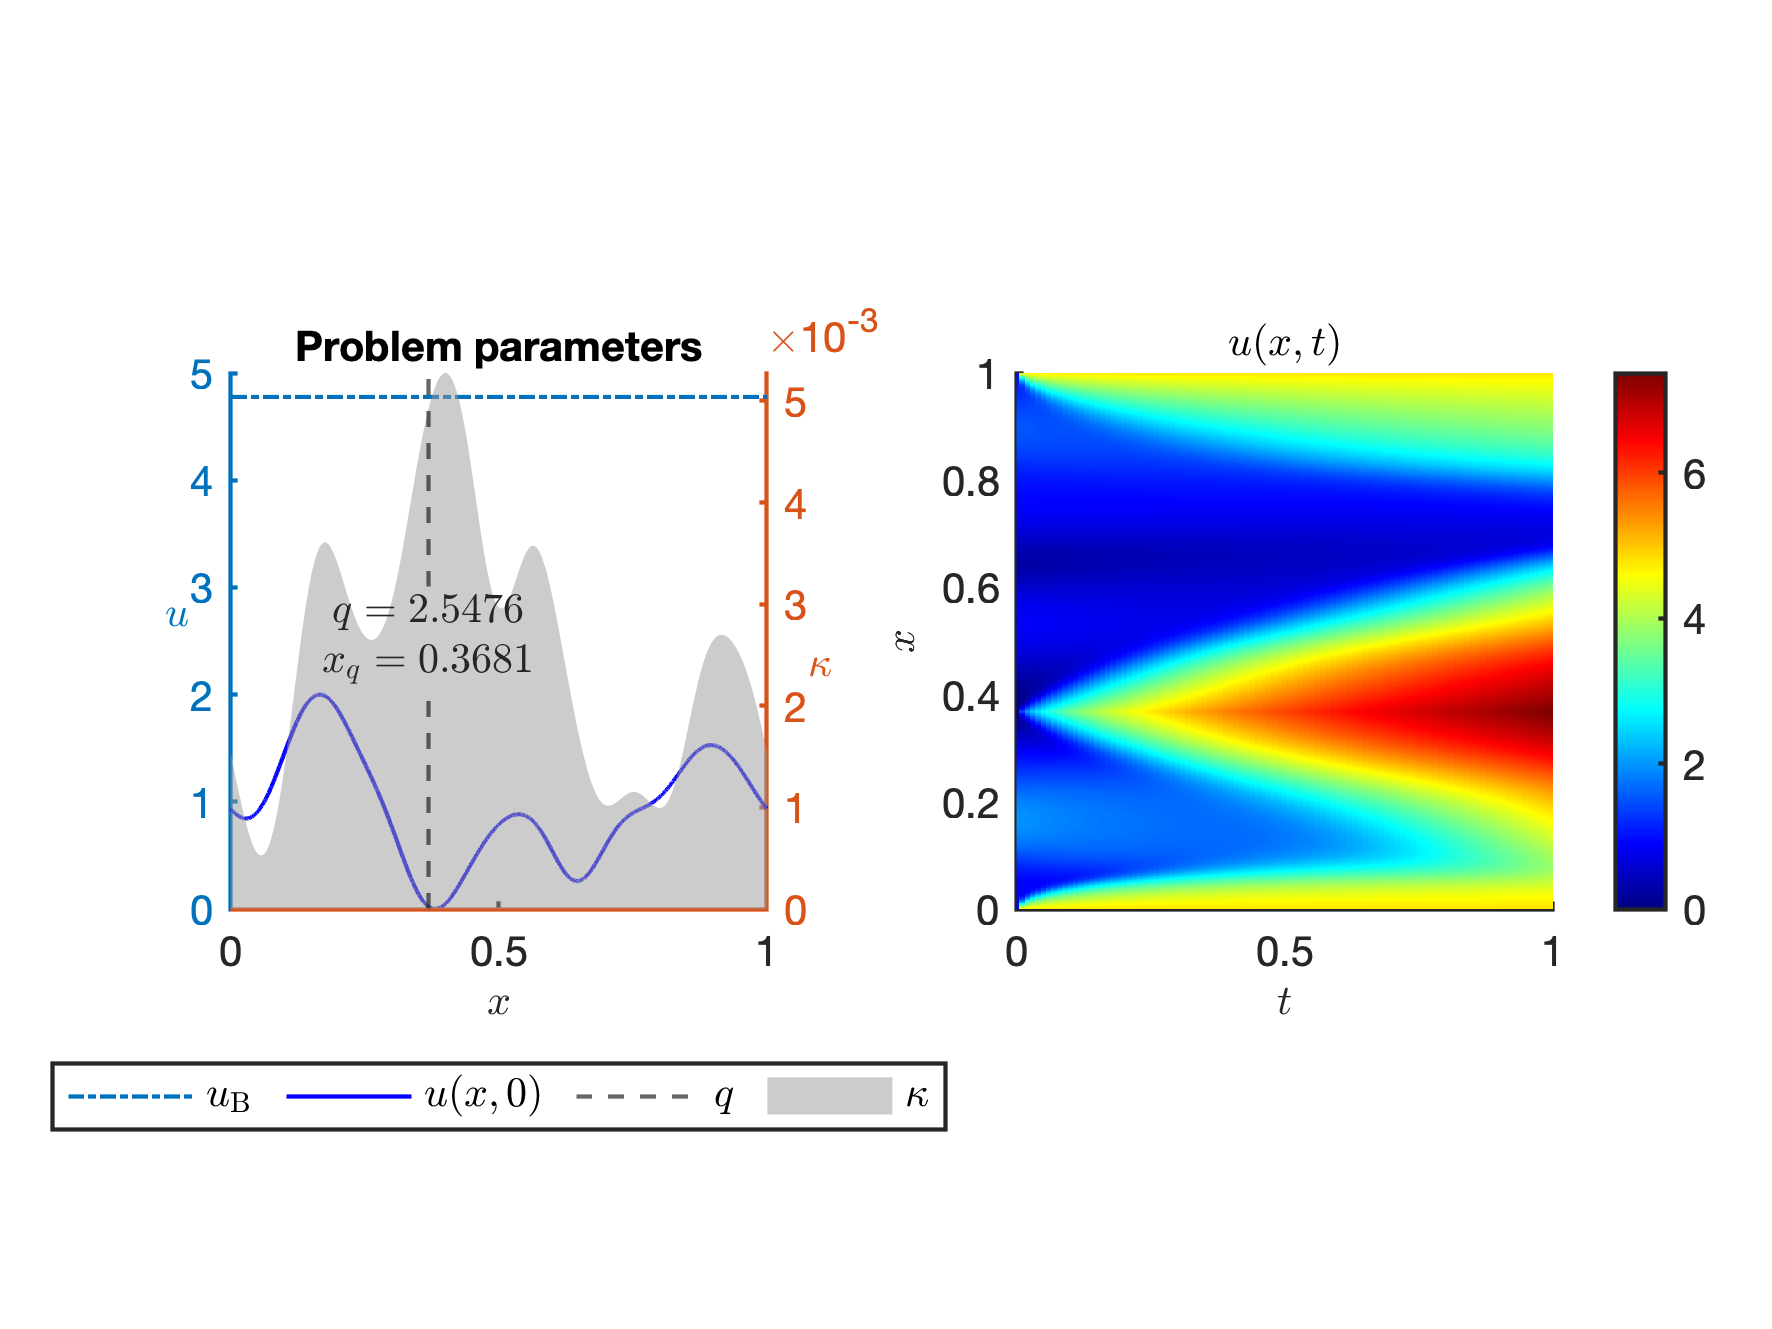
\includegraphics[width=\textwidth,trim={0 1.5cm 0 2.5cm},clip]{./sci_report/images/ECMOR/1-FOM.png}
    }
    \caption{Пример постановки задачи \ref{eq:diffusion} с симметричным граничным условием Дирихле $u_\text{B}$ и её численного решения \cite{Elizarev2022}}\label{fig:FOM}
\end{figure}


\section{Методы анализа данных для снижения размерности}

В данном разделе приведены используемые в работе основные методы эмпирического снижения размерности и соответствующие выдвигаемые положения.

\subsection{Снижение размерности нелинейной модели}

Рассматривается задача решения системы нелинейных алгебраических уравнений, соответствующая поиску численного решения определяющего уравнения на том или ином временном шаге.

\begin{align}
    \unk_\ast : \resid(\unk_\ast) = 0 \\
   \unk_\ast = \arg \min_{\unk} \norm{\resid(\unk)}
\end{align}

В качестве метода решения нелинейной системы рассматривается метод Ньютона и соответствующая детерминированная линейная задача, решаемую на итерациях этого метода. Вычислительная сложность линейной задачи растёт полиномиально с $\dim \unk$.
\begin{align}
    \resid(\unk + \Delta \unk) \approx \resid(\unk) + \jac(\unk) \dunk ,\; \jac = \deriv{\resid}{\unk}\\
    \dunk_\ast (\unk) = \arg \min_{\dunk} \norm[2]{\resid(\unk) + \jac(\unk) \dunk} \label{eq:du}\\
    \jac(\unk) \dunk_\ast = - \resid(\unk)
\end{align}

Далее рассматривается абстрактное линейное подпространство с ортогональным базисом $\Phi^{-1} = \transpose{\Phi}$ в качестве аппроксимирующей замены переменной $\unk_\Phi (\vunk) = \Phi \vunk$ такой, что $\dim{\vunk} \leq \dim{\unk}$. Качество аппроксимации количественно измеряется с помощью евклидовой нормы $\norm[2]{\unk_\Phi - \unk}$.

% \begin{align}
%     \unk_\Phi (\vunk) = \Phi \vunk \\
%     \dim{\vunk} \leq \dim{\unk} \\
%     \norm{\unk_\Phi - \unk} \\
%     \Phi^{-1} = \transpose{\Phi}
% \end{align}

Подстановка переменных $\vunk$ в линейную задачу \ref{eq:du} приводит к линейной задаче, переопределенной в общем случае.
\begin{align}
    \dvunk_\ast = \arg \min_{\dvunk} \norm[2]{\resid(\Phi \vunk) + \jac(\Phi \vunk) \Phi \dvunk} \label{eq:dv}\\
    \transpose{P}\jac \dvunk_\ast = - \transpose{P} \resid \label{eq:dv-projected}
\end{align}

Проекция на $\matr{P} \in \mathbb{R}^{\dim \unk \times \dim \vunk}$ в уравнении \ref{eq:dv-projected} формирует детерминированную задачу.
В качестве $\matr{P}$ рассматриваются проекция Галеркина $\matr{P}_\text{G}$ и проекция для задачи наименьших квадратов $\matr{P}_\text{LS}$.
% В последнем случае метод решения нелинейной системы эквивалентен методу Ньютона --- Гаусса для переопределённых систем.
\begin{align}
    \matr{P}_\text{G} = \Phi \\
    \matr{P}_\text{LS} = \jac \Phi \\
\end{align}

Результат соответствующего итерационного процесса $\vunk_\ast$ характеризуется тем, что норма невязки в этом процессе в общем случае сходится к положительному значению в отличие от полноразмерной детерминированной задачи. При этом норма спроецированной невязки в сходящемся процессе сходится к нулю.
\begin{align}
    \norm{\resid(\Phi \vunk_\ast)} \geq 0\\
    \norm{\transpose{P}\resid(\Phi \vunk_\ast)}
\end{align}

Предлагается следующее решение для оценки сходимости низкоразмерной задачи.
Пусть для нормированной невязки полноразмерной задачи в качестве критерия сходимости выбрано значение $\varepsilon > 0$. Пусть также низкоразмерная задача решается в проекции на $\matr{P}_{\text{LS}}$ как наиболее предпочтительной.
\begin{equation}
    \varepsilon_\text{FOM} = \norm{\frac{\resid}{\dim{\resid}}} \leq \varepsilon \\
\end{equation}
Кроме того, делается предположение о том, что в соответствующем процессе сходится к нулю и спроецированная на $\norm{\transpose{P}_\text{G}\resid}$. Тогда для сопоставления сходимости низкоразмерных и низкоразмерных задач предлагается использовать следующий критерий вне зависимости от выбранной для итерационного процесса проекции.
\begin{equation}
    \varepsilon_\text{ROM} = \norm{\frac{\transpose{\matr{P}_\text{G}}\resid}{\dim{ \transpose{\matr{P}_\text{G}}\resid}}} \leq \varepsilon
\end{equation}

\subsection{Правильное ортогональное разложение}

Рассматривается абстрактная динамическая задача конечной размерности $N_\unk = \dim \unk$ с начальным условием $\unk_0$ и параметрами $\param$.
\begin{equation}
    \unk_n = \arg \min_{\unk} \norm{\resid_n(\unk,\unk_{n-1};\param)}
\end{equation}

Метод правильного ортогонального разложения, также известного как метод главных компонент, использует последовательность решений $\unk_n$ как выборку, формирующую матрицу данных $\matr{U} (\param)$.
\begin{align}
    \unk_\text{o} (= \unk_0) \\
    \matr{U} (\param) =
    \begin{bmatrix}
        \unk_0, \unk_1, \dots, \unk_{N_t}
    \end{bmatrix}
\end{align}

Далее возможно сместить выборку на $\unk_\text{o}$ (равное, например, начальному условию $\unk_0$) и рассмотреть левые сингулярные вектора из соответствующего разложения, упорядоченного по убыванию сингулярных чисел.
\begin{align}
    \matr{u} - \unk_\text{o} = \Phi \Sigma \transpose{\Upsilon} \\
    \Phi^{-1} = \transpose{\Phi} \\
    \Phi = \begin{bmatrix}
        \widetilde{\Phi}, \pc[N_\vunk + 1], \dots
    \end{bmatrix}
\end{align}
Усеченный набор главных компонент (сингулярных векторов) формирует эмпирическую линейную замену переменных $\widetilde{\Phi}$.
\begin{align}
    \unk_{\widetilde{\Phi}} = \widetilde{\Phi} \vunk \\
    \unk_{\widetilde{\Phi}}(\unk) = \widetilde{\Phi} \transpose{\widetilde{\Phi}} \unk
\end{align}

\begin{figure}[ht]
    \centerfloat{
        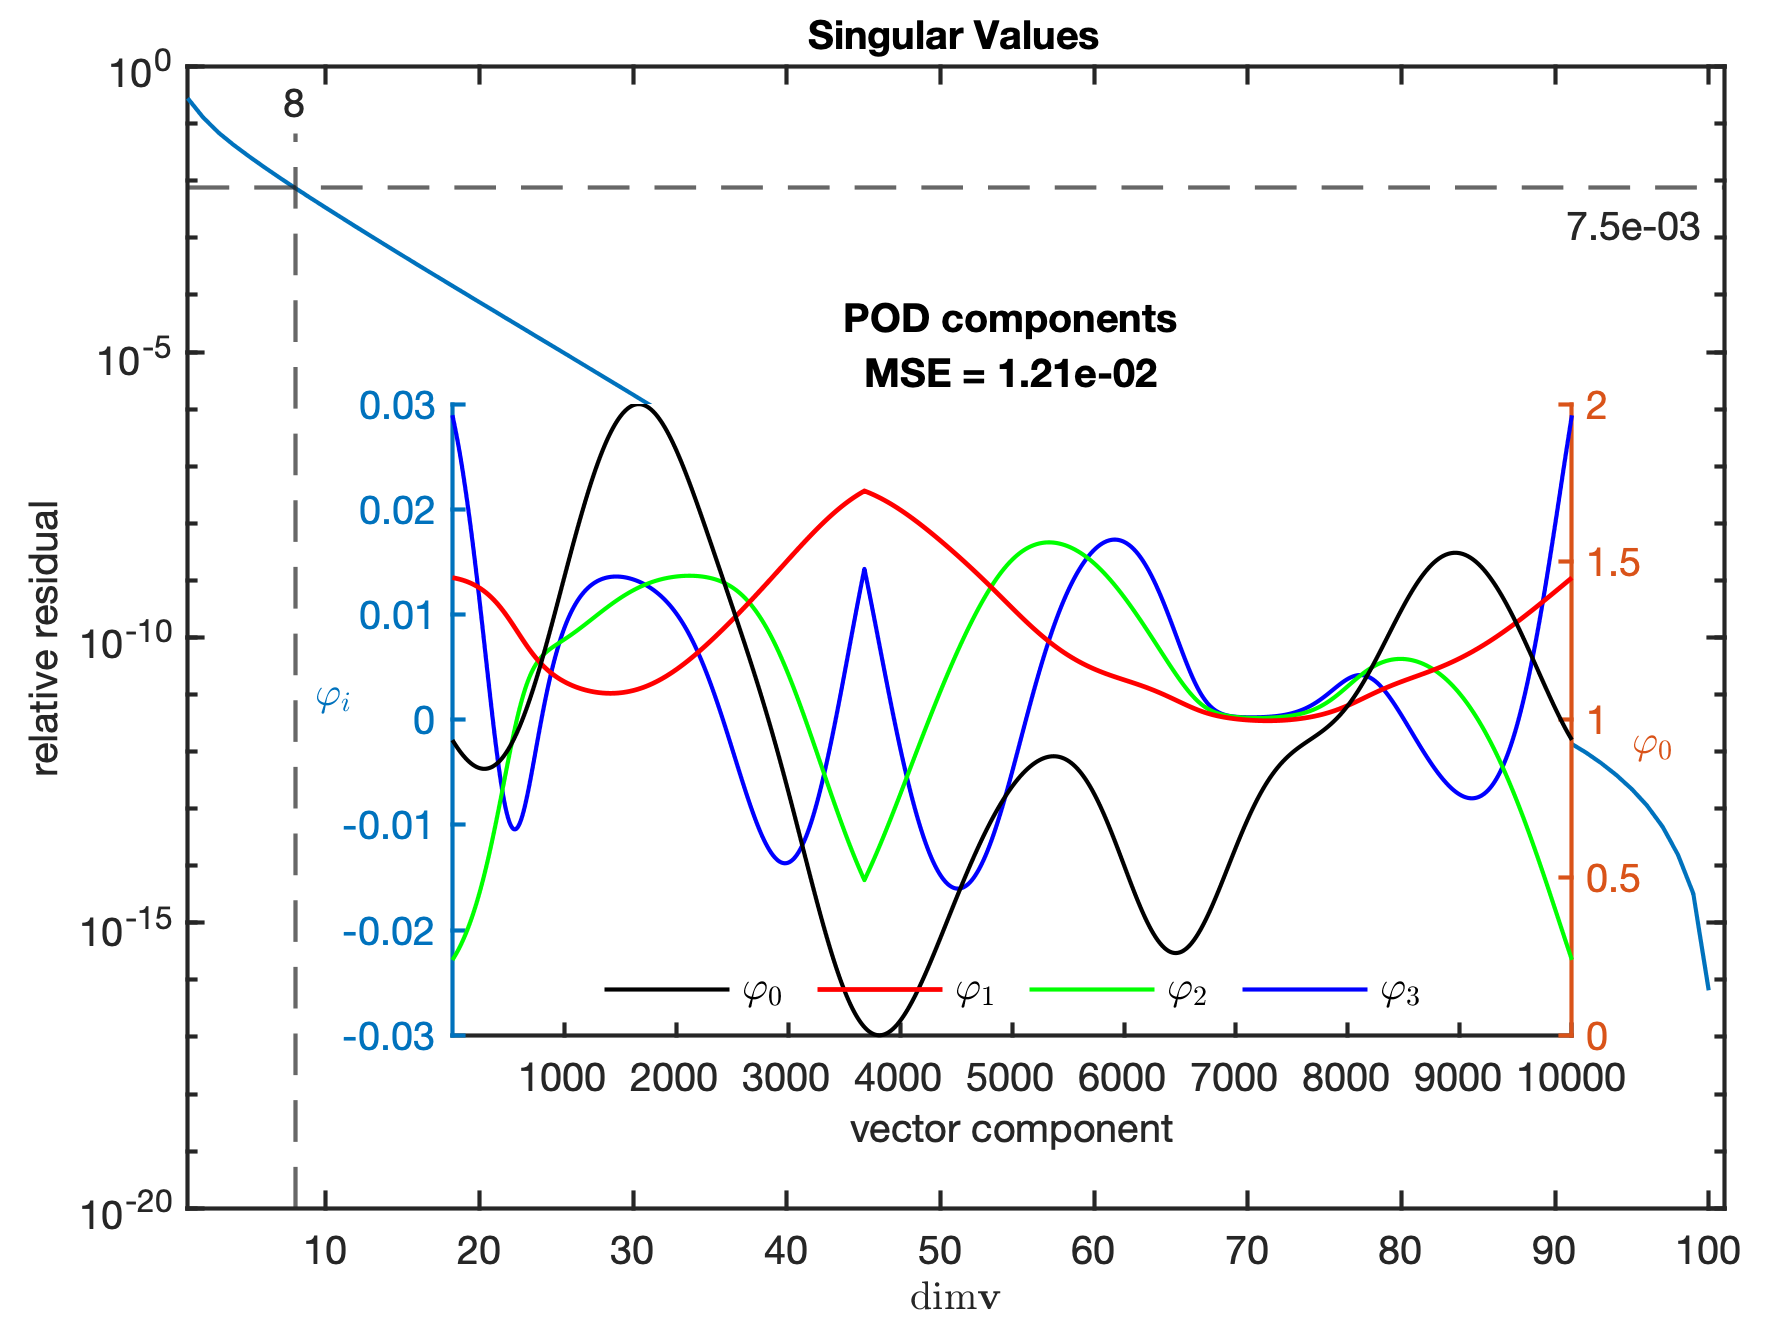
\includegraphics[scale=1]{./sci_report/images/ECMOR/2-POD.png}
    }
    \caption{Пример базисных векторов правильного ортогонального разложения для модельной задачи \ref{eq:diffusion}~\cite{Elizarev2022}}\label{fig:POD}
\end{figure}

Одним из основных аспектов применимости эмпирического снижения размерности является репрезентативность извлечённых главных компонент для произвольной точки в пространстве параметров $\param$ и достаточность малого количества главных компонент для желаемой точности низкоразмерного расчёта.

\begin{figure}[ht]
    \centerfloat{
        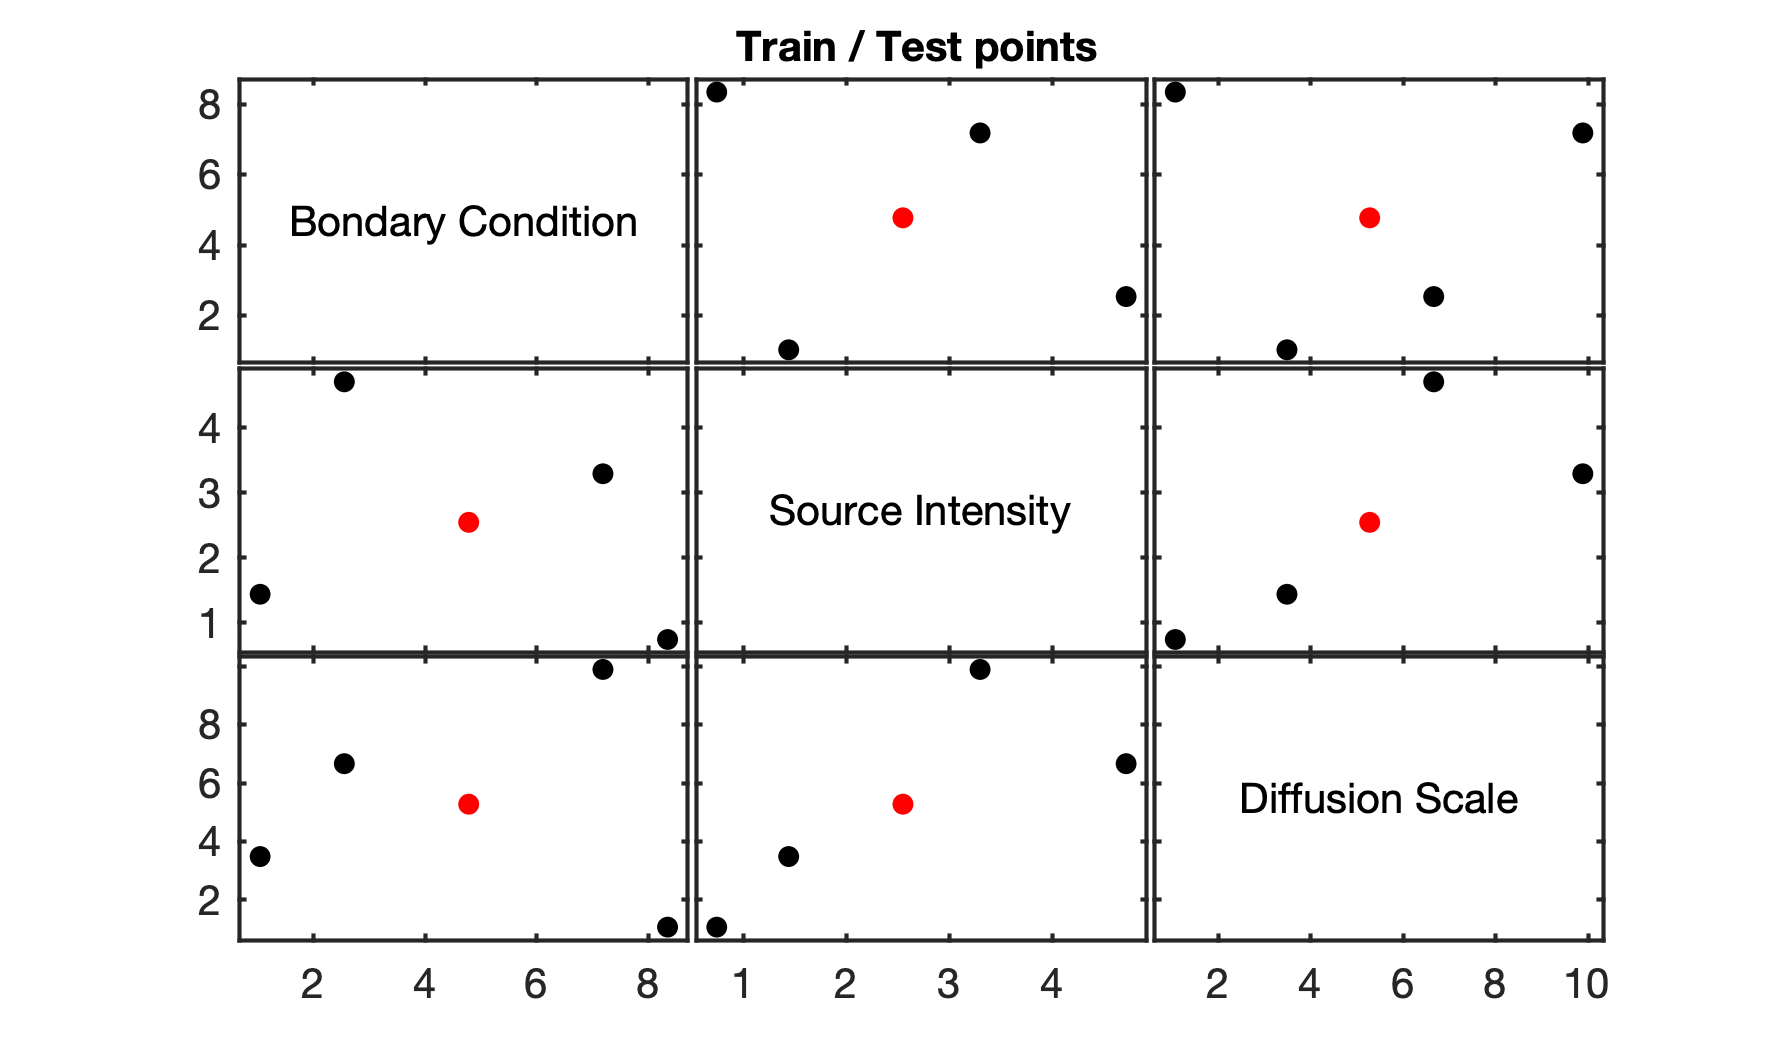
\includegraphics[scale=1]{./sci_report/images/ECMOR/6-Train-Test.png}
    }
    \caption{Пример элементов обучающей выборки (чёрные точки) и тестовой (красной) точки в пространстве параметров модельной задачи~\cite{Elizarev2022}}\label{fig:params}
\end{figure}

\begin{align}
    \matr{M} =\begin{bmatrix}
        \param_1, \dots, \param_{N_\param}
    \end{bmatrix} \label{eq:param-space}\\
    \matr{U}(\matr{M}) =
    \begin{bmatrix}
        \matr{U}(\param_1), \dots, \matr{U}(\param_{N_\param})
    \end{bmatrix}
    \rightarrow \widetilde{\Phi (\matr{M})} \label{eq:param-concat}\\
    \widetilde{\Phi} (\matr{M}) \matr{R}_\text{qr} =
    \begin{bmatrix}
        \widetilde{\Phi}(\param_1), \dots,  \widetilde{\Phi}(\param_{N_\param})
    \end{bmatrix} \label{eq:param-pod-qr}
\end{align}

Для точек обучающей выборки $\matr{M}$ в уравнении \ref{eq:param-space} рассматриваются альтернативные варианты построения главных компонент.
Вариант в соотношении \ref{eq:param-concat} предполагает извлечение главных компонент из конкатенации матриц данных, в то время как соотношение \ref{eq:param-pod-qr} соответствует конкатенации независимых наборов главных компонент с дополнительно произведенной ортогонализацией.
Предпочтение отдаётся второму варианту как требующего меньшего количества вычислений и потребления памяти при формировании главных компонент по выбранному набору точек в пространстве параметров.
% \begin{equation}
% N_\vunk : \widetilde{\Phi} \in \mathbb{R}^{N_\unk \times N_\vunk}
% \end{equation}

\begin{figure}[ht]
    \centerfloat{
        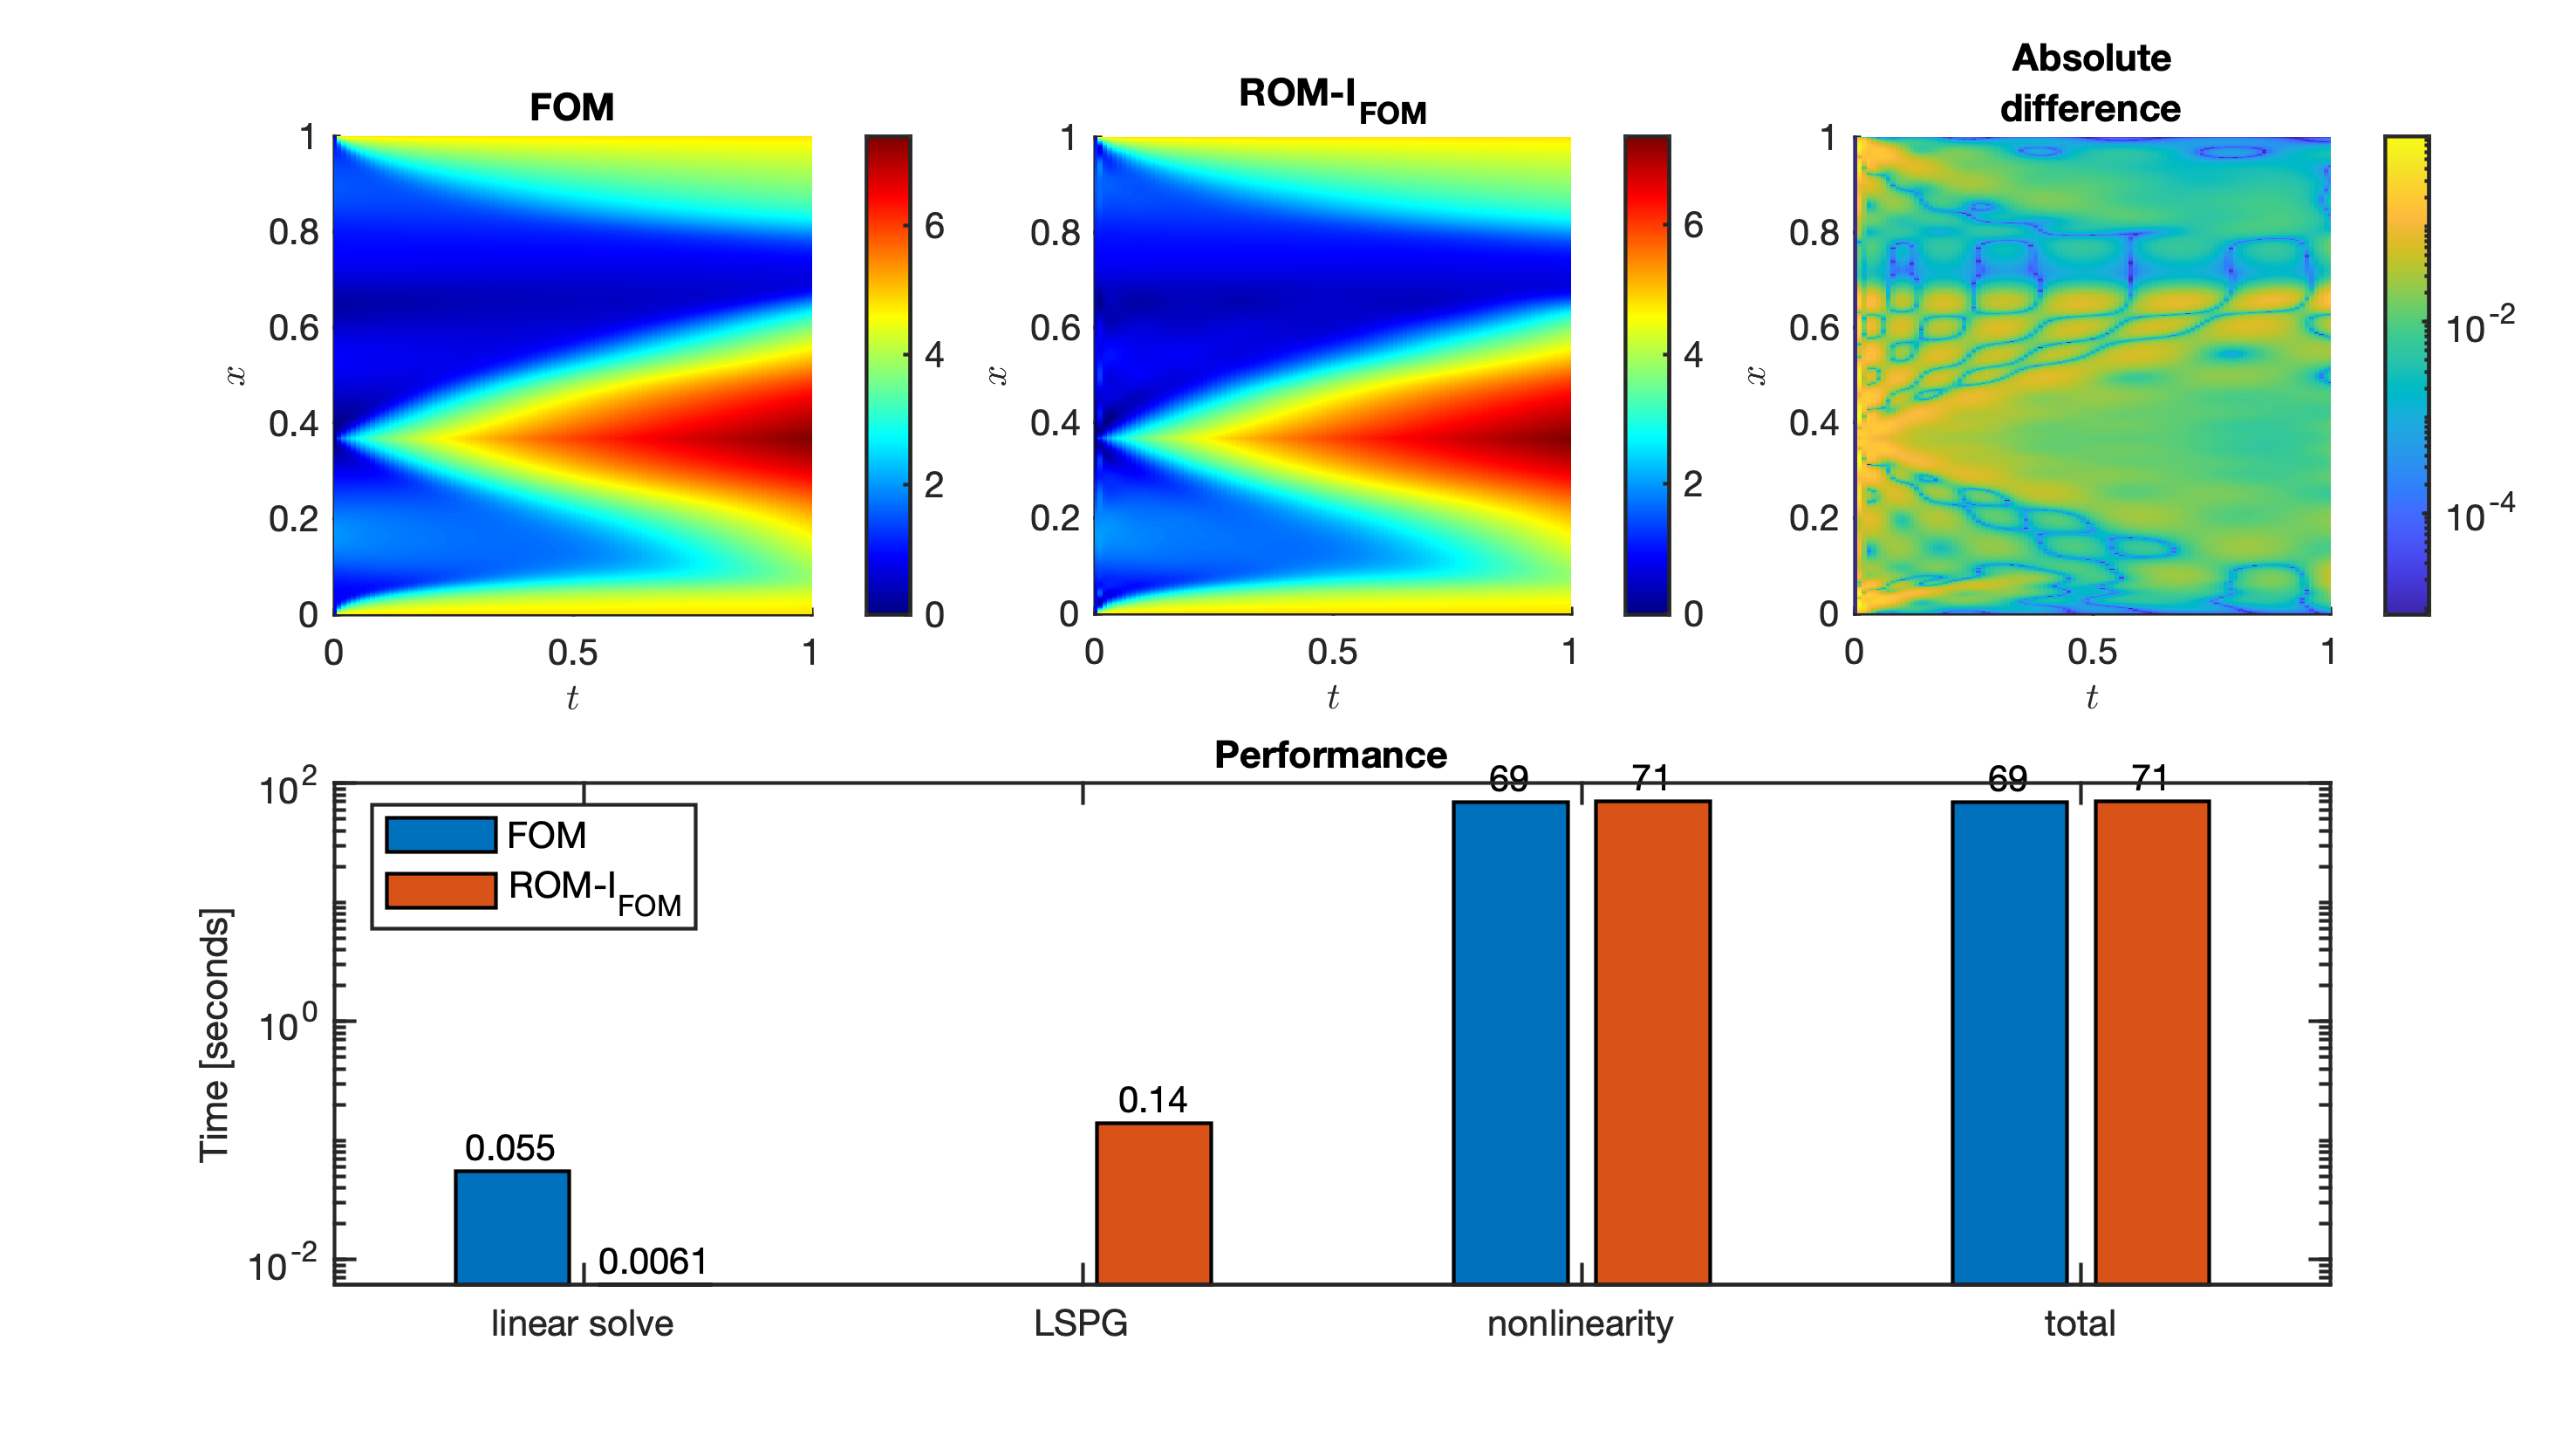
\includegraphics[width=\textwidth]{./sci_report/images/ECMOR/3-ROM-I.png}
    }
    \caption{Пример ускорения решения линейной задачи с помощью правильного ортогонального разложения~\cite{Elizarev2022}}\label{fig:ROM-I}
\end{figure}

\subsection{Аппроксимация нелинейных функций высокой размерности}

На Рисунке~\ref{fig:ROM-I} в том числе отражена проблематика снижения размерности нелинейных моделей: Количество нелинейных вычислений, на которые может приходиться значительная доля времени решения полноразмерной задачи, не сокращается вместе с размерностью пространства неизвестных. В данном подразделе рассматривается метод эмпирической интерполяции нелинейных функций, так же использующий правильное ортогональное разложение.

Рассматривается аналогичная выборка нелинейных функций высокой размерности $\nlin$, формируются главные компоненты $\widetilde{\Phi}_\mathcal{N}$.
\begin{align}
    \nlin(\unk) \rightarrow \nlin (\unk_{\widetilde{\Phi}}) = \nlin (\widetilde{\Phi} \vunk),~\dim{\nlin} \sim \dim{\unk} \\
    \mathcal{N} =
    \begin{bmatrix}
        \nlin_1, \dots,  \nlin_{N_\nlin}
    \end{bmatrix} \\
    \mathcal{N} \rightarrow \widetilde{\Phi}_\mathcal{N} \\
    \nlin \approx \widetilde{\Phi}_\mathcal{N} \bvec{\gamma}
\end{align}
Далее выбирается $N_{\bvec{\rho}} < \dim{\nlin}$ компонент вектора $\nlin$, вычисляемых непосредственно. Соответствующее подпространство компонент $P$ назовём подпространством нелинейных измерений, в котором непосредственно вычисленные компоненты формируют вектор $\overline{\nlin}$.
\begin{align}
   \bvec{\rho} : \rho_m \in \left\{0, 1 \right\},~N_{\bvec{\rho}} = \sum_m \rho_m \\
   \overline{\nlin} = \transpose{P} \nlin,~\matr{P} \in \mathbb{R}^{\dim{\nlin} \times N_{\bvec{\rho}}}
\end{align}

\begin{figure}[ht]
    \centerfloat{
        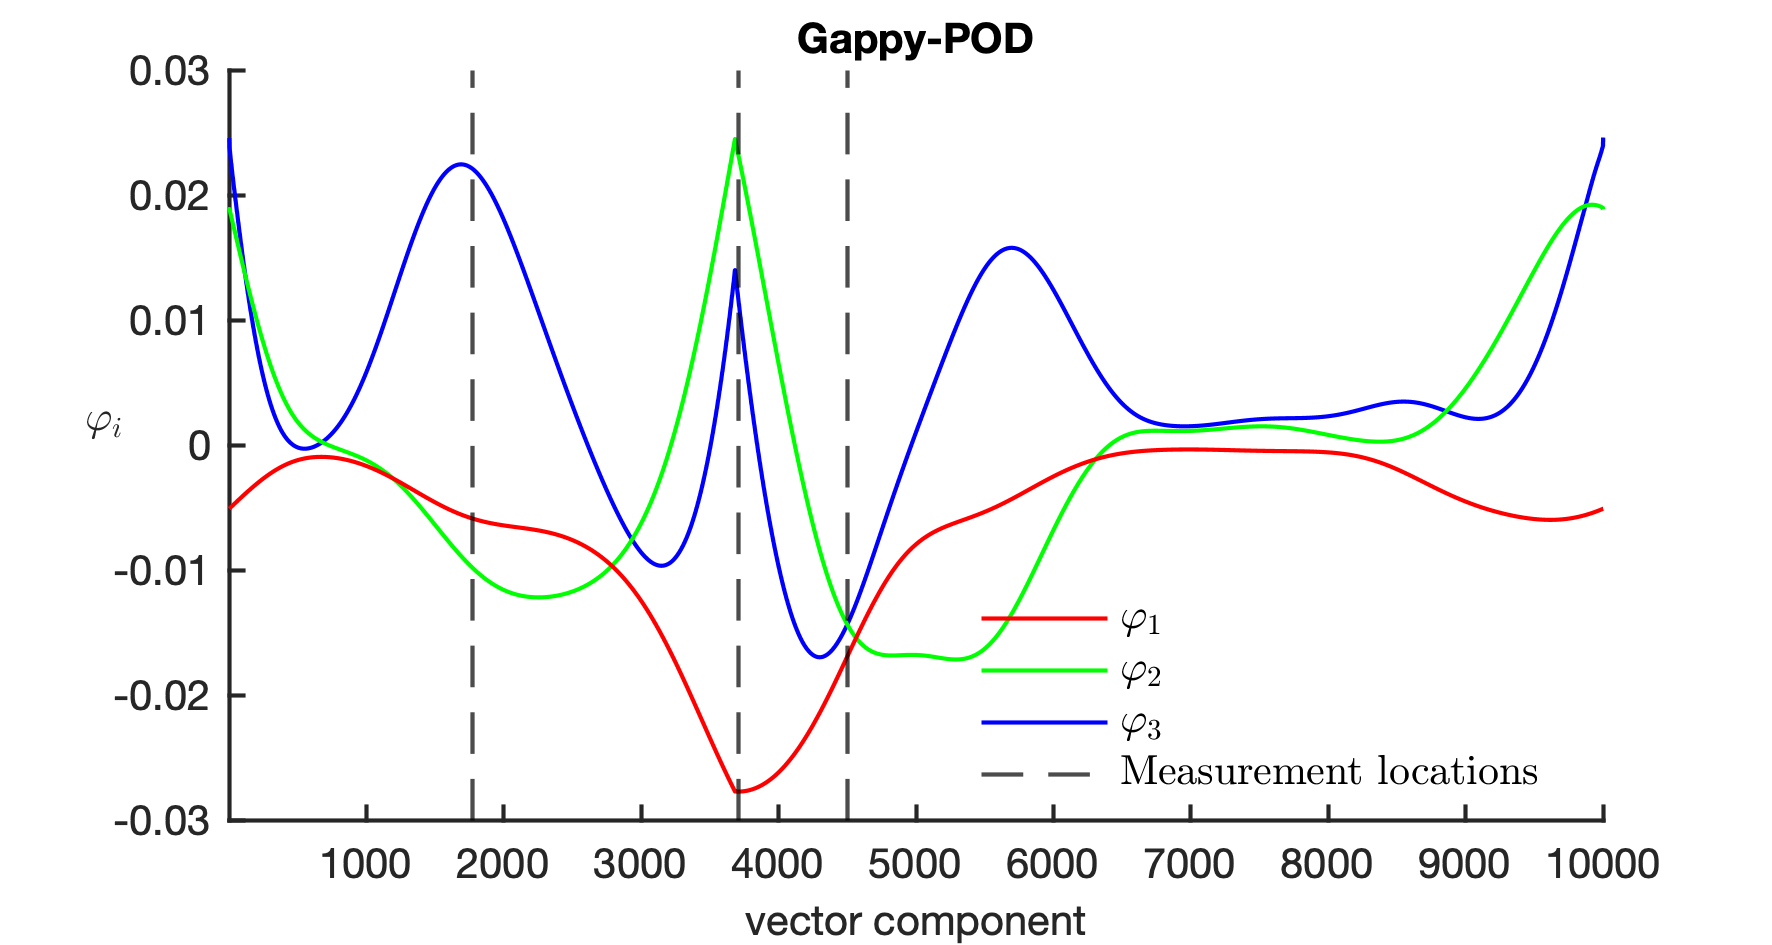
\includegraphics[scale=1]{sci_report/images/ECMOR/4-Gappy.png}
    }
    \caption{Пример главных компонент нелинейных функций и выбранного подпространства нелинейных изменений (вертикальные штрихи)~\cite{Elizarev2022}}\label{fig:gappy}
\end{figure}

Для вычисления эмпирической интерполяции поиск вектора в пространстве главных компонент, максимально соответствующего вычисленным значениям $\overline{\nlin}$ при его проекции на пространство нелинейных измерений. Решение соответствует операции косой проекции $\mathcal{O}$ из $\widetilde{\Phi}_\mathcal{N}$ на $\matr{P}$ ортогонально последнему.
\begin{align}
    \widehat{\bvec{\gamma}} = \arg \min_{\bvec{\gamma}} \norm[2]{\transpose{P} \widetilde{\Phi}_\mathcal{N} \bvec{\gamma} - \overline{\nlin}} \\
    \widehat{\bvec{\gamma}} = {\left( \transpose{P} \widetilde{\Phi}_\mathcal{N} \right)}^\dagger \overline{\nlin} = \mathcal{O} \overline{\nlin} \\
    \widehat{\nlin} = \widetilde{\Phi}_\mathcal{N} \widehat{\bvec{\gamma}} = \matr{\Pi} \overline{\nlin}
\end{align}
При подстановке аппроксимированных нелинейных функций в задачу \ref{eq:dv} формируется низкоразмерная модель следующего уровня.
\begin{align}
    \dvunk_\ast (\vunk)= \arg \min_{\dvunk} \norm[2]{\widehat{\resid}(\Phi \vunk) + \widehat{\jac}(\Phi \vunk) \Phi \dvunk}
\end{align}
Также отмечается важная особенность аппроксимации нелинейных функций. Предлагается не включать в аппроксимируемые функции линейные операции, в том числе соответствующие конечно-разностным аппроксимациям производных. Такой подход сохраняет характерные и необходимые для многих численных методов свойства возникающих матриц и позволяет заранее предварительно рассчитывать матричные произведения с оператором косой проекции.
\begin{align}
    \matr{\matr{L}} \nlin \approx
    \matr{\matr{L}} \matr{\Pi} \overline{\nlin} = \widehat{\matr{\matr{L}}} \overline{\nlin}
\end{align}

\begin{figure}[ht]
    \centerfloat{
        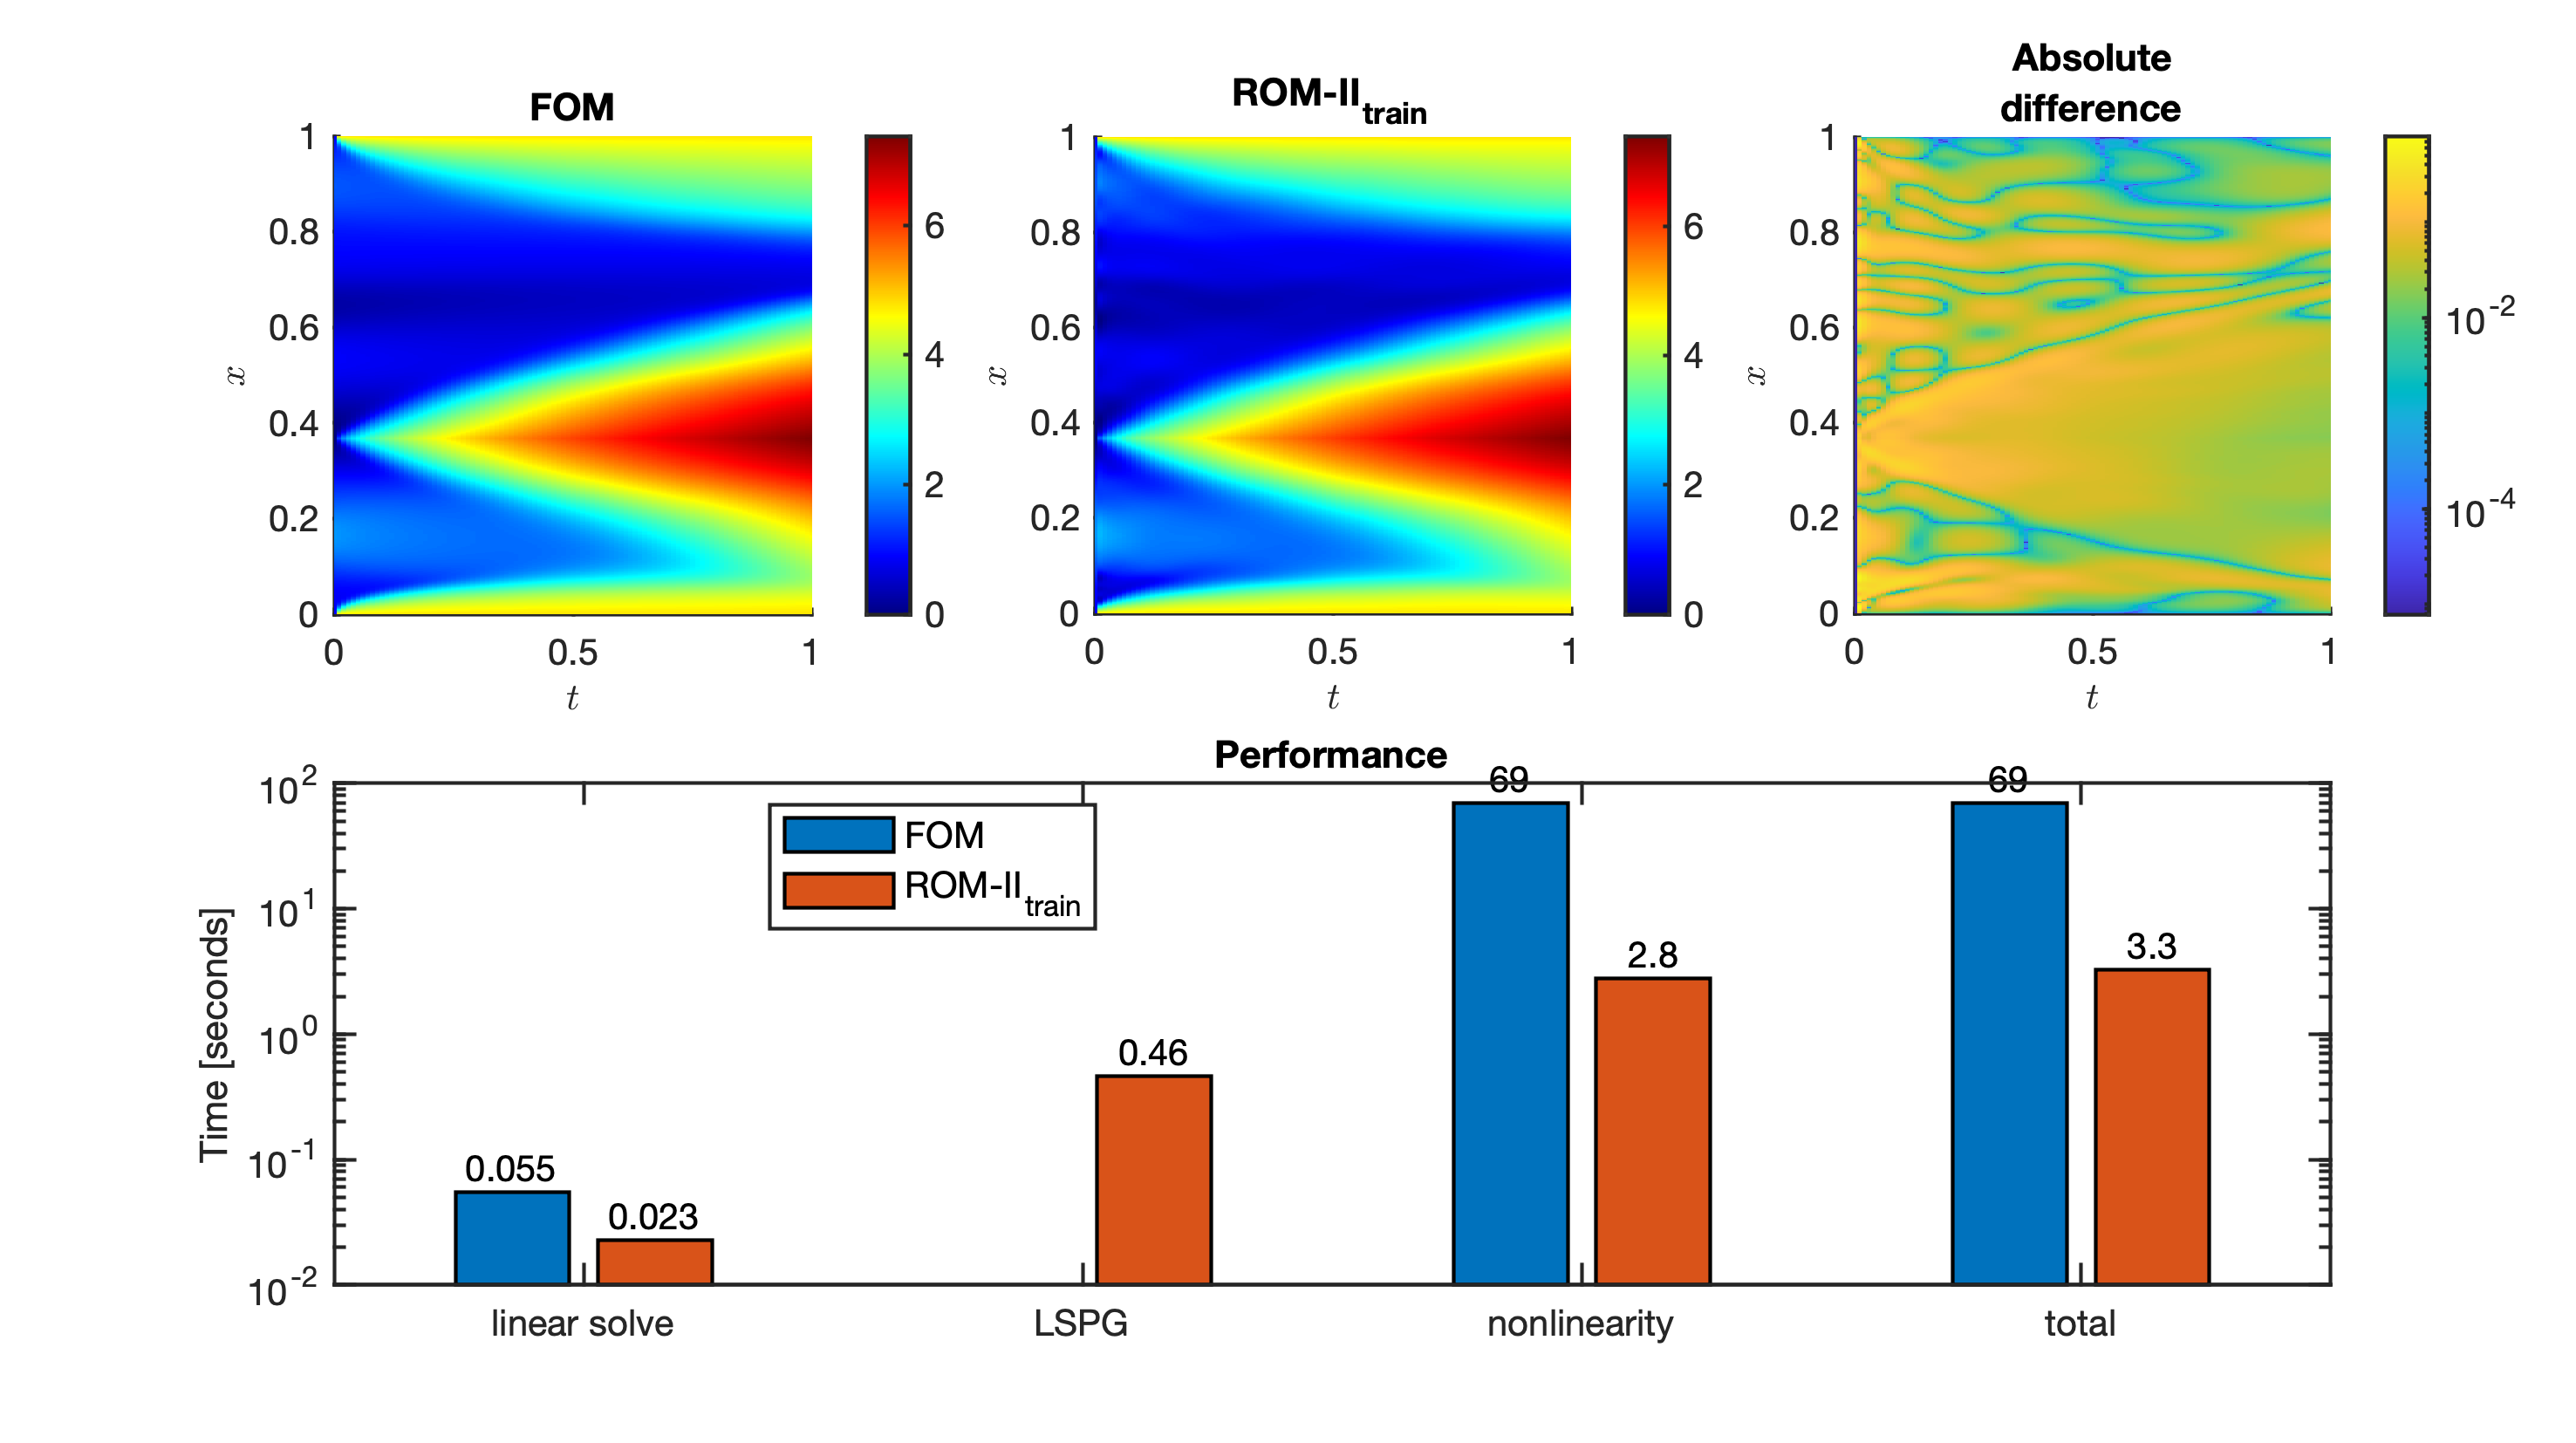
\includegraphics[width=\textwidth]{./sci_report/images/ECMOR/7-ROM-II-Train.png}
    }
    \caption{Пример ускорения, достигаемого при низкоразмерном моделировании с эмпирической интерполяцией нелинейных функций~\cite{Elizarev2022}}\label{fig:ROM-II}
\end{figure}

% \subsection{Использование данных для предобуславливания}

% \begin{equation}
%     \unk_{n+1} \approx \matr{D} \unk_{n}
% \end{equation}

% \begin{align}
%     \matr{U}_{-} &=
%     \begin{bmatrix}
%         \unk_0, \dots, \unk_{N_t-1}
%     \end{bmatrix}\\
%     \matr{U}_{+} &=
%     \begin{bmatrix}
%         \unk_1, \dots, \unk_{N_t}
%     \end{bmatrix}
% \end{align}

% \begin{align}
%     \matr{D} = \arg \min_{\matr{A}} \norm[\text{fro}]{\matr{U}_{+} - \matr{D} \matr{U}_{-}} = \matr{U}_{+} \matr{U}_{-}^{\dagger}
% \end{align}

% \begin{align}
%     \widetilde{\Phi} \vunk_{n+1} \approx  \matr{D} \widetilde{\Phi} \vunk_{n} \\
%     \vunk_{n+1} \approx  \matr{D}_{\widetilde{\Phi}} \vunk_{n} \\
% \end{align}

% \begin{align}
%     \left\{ \Psi_{\widetilde{\Phi}},  \widetilde{\Lambda} \right\} : \matr{D}_{\widetilde{\Phi}}  \Psi_{\widetilde{\Phi}} = \Psi_{\widetilde{\Phi}} \widetilde{\Lambda} \\
%     \widetilde{\Psi} = \widetilde{\Phi} \Psi_{\widetilde{\Phi}} \widetilde{\Lambda} \\
%     \matr{D} \widetilde{\Psi} = \widetilde{\Psi}\widetilde{\Lambda} \\
%     \left\{\widetilde{\Psi},  \widetilde{\Lambda} \right\} \rightarrow \widetilde{\matr{D}}\\
%     \unk_{n+1} \approx \widetilde{\matr{D}} \unk_{n}
% \end{align}

% \begin{align}
%    \unk \rightarrow \nlin(\unk) \rightarrow \matr{D}_{\nlin}
% \end{align}

% \begin{align}
%     \exists \nlin(\unk), \matr{\mathcal{K}} : \nlin_{n+1} \equiv \matr{\mathcal{K}}  \nlin_{n}
%  \end{align}

% \begin{align}
%     \unk_{n+1} \approx \matr{D} \unk_{n} + \matr{B} \bvec{q}_{n} + \matr{C} \bvec{q}_{n+1}
% \end{align}

% \subsection{{Иерархия эмпирических методов ускоренного моделирования}}

\begin{figure}[ht]
    \centerfloat{
        \includegraphics[width=\textwidth]{./sci_report/images/seminar/ROM-ROM-3.png}
    }
    \caption{Диаграмма условных уровней эмпирического низкоразмерного моделирования}\label{fig:ROM-II}
\end{figure}

% \subsubsection{{Накопление данных в итеративных прямых расчётах}}

% multi-level Monte Carlo
